\section{Model of Cart and Inverted Pendulum \label{sec:pen_model}}
In this section, a model of the inverted pendulum is derived. This model describes the movement of the cart and the inverted pendulum, based on governing equations put up regarding the behaviour of the system. To do this, it is necessary to investigate how the inverted pendulum moves, and how the interaction between the inverted pendulum and the cart can be described. Before this is done in detail, it is however first necessary to obtain an overview of the inverted pendulum.
\subsection{Overview of the Inverted Pendulum}
The model of the inverted pendulum describes how the two masses, i.e. the cart and the inverted pendulum, behaves when a force is exerted upon it by the surroundings. Note that the rod connecting the inverted pendulum mass to the cart is assumed massless, and is therefore not a part of the model. A schematic drawing of the inverted pendulum is shown in \autoref{fig:mecmodinvpen}.
\begin{figure}[H]
\centering
%\includegraphics[scale=1]{needstobechaged1.png}
\scalebox{0.6}{\input{figures/invpenmec.ralf}}
\caption{Mechanical model of the inverted pendulum.}
\label{fig:mecmodinvpen}
\end{figure}
In \autoref{fig:mecmodinvpen} the mass at the end of the rod is $m_p$, the variable $\theta_p(t)$ describes the angle of the inverted pendulum from a vertical line at the center of the cart. Note that the angle is positive in the counter-clockwise direction. This angle can be described in relation to both the x- and y-direction. The force applied to move the segway is labelled $F_F(t)$.\\\\
For simplicity, the coordinate system is defined such that $y_c(t)$ is 0, thus:
\begin{align}
x_p(t)&= x_c(t)- l \cdot \sin(\theta_p(t))\\
y_p(t)&= l\cdot \cos(\theta_p(t)) 
\end{align}
\begin{where}
\va{$x_p(t)$}{is the x-position of the inv. pendulum}{m}\\
\va{$x_c(t)$}{is the x-position of the cart}{m}\\
\va{$l$}{is the length between the center of rotation of the cart and the center of mass of the inv. pendulum}{m}\\
\va{$\theta_p(t)$}{is the angle of the inv. pendulum}{rad}\\
\va{$y_p(t)$}{is the y-position of the inv. pendulum}{m}\\
\end{where}

From this, the accelerations can be found by taking the double time differential of both sides of the above equations:
\begin{align}
\ddot x_p(t) &= \ddot x_c(t) + l \cdot \sin(\theta_p(t))\cdot \dot\theta_p^2 (t) - l \cdot \cos(\theta_p(t))\cdot \ddot\theta_p(t) \label{eq_acc_x}\\
\ddot y_p(t) &= -l\cdot \cos(\theta_p(t)) \cdot \dot\theta_p^2 (t) - l \cdot \sin(\theta_p(t))\cdot \ddot\theta_p (t)\label{eq_acc_y}
\end{align}
\begin{where}
\va{$\ddot x_p(t)$}{is inv. pendulum's acceleration in the x-direction }{rad/$\text{s}^2$}\\
\va{$\ddot \theta_p(t)$}{is inv. pendulum's angular acceleration}{rad/$\text{s}^2$}\\
\va{$\dot \theta_p(t)$}{is inv. pendulum's angular velocity}{rad/s}\\
\va{$\ddot y_p(t)$}{is inv. pendulum's acceleration in the y-direction }{rad/$\text{s}^2$}\\
\end{where}
%To make a transfer function for the inverted pendulum that can be merged with the transfer function for the motors and wheels, an equation in time domain describing the change in $\theta_p(t)$ caused by any $F_F(t)$ must first be derived. This is done in the following section.

To derive a model expression for the inverted pendulum, which shall be combined with a model expression for the motors and wheels, an equation %in time domain 
 describing the change in $\theta_p(t)$ caused by any $F_F(t)$ must first be derived. This is done in the following section.
\subsection{Equations of Motion}
In this section, translatoric free body diagrams for the cart and the inverted pendulum are presented and used to derive equations of motion. From these, a model of the cart and the inverted pendulum can be obtained.
 %\todo{is it still the only purpose, i think it has changed.A}The goal of this section is to arrive at one expression with only two variables, namely the input, $F_F(t)$ and the output, $\theta_p(t)$ of the model for the inverted pendulum. %Subsequently this expression is verified through simulation, and comparison with expected result.
\newpar
From \autoref{fig:mecmodinvpen}, free body diagrams can be determined. In this case, the cart's and the inverted pendulum's free body diagrams are representing the forces acting upon them while the segway is at an angle, $\theta_p(t)$.\\
The free body diagram of the mass at the end of the rod, is shown in \autoref{fig:fbdm1}.
\begin{figure}[H]
%\hspace{-0.5 cm}
\centering
\begin{subfigure}[b]{0.42\textwidth}
		\hspace{1.5cm}
        \scalebox{0.6}{\input{figures/invpen_M2_FBD.ralf}}
        %\vspace{3mm}
		\caption{FBD of the cart.}
		\label{fig:fbdm2}
\end{subfigure}
\hspace{1 cm}
\begin{subfigure}[b]{0.42\textwidth}
		\centering
        \scalebox{0.6}{\input{figures/invpen_M1_FBD.ralf}}
        %\vspace{10 mm}		
		\caption{FBD of the pendulum mass.}
		\label{fig:fbdm1}
    \end{subfigure}  
\caption{Free body diagrams of the mass of the inverted pendulum and the mass of the cart.}
\label{fig:FBDMotorWheel}
\end{figure}
\clearpage
The forces acting on the the mass $m_p$ is the gravitational force $F_g$, and the tension in the rod between the cart and the inverted pendulum, $F_t(\theta_p(t))$. This force is split up into two composants - a composant in the x-direction, $F_{tx}(\theta_p(t))$ and one in the y-direction, $F_{ty}(\theta_p(t))$. % The magnitude of this force depends on the angle, $\theta_p(t)$.\\
\autoref{fig:fbdm2} shows the free body diagram of the segway's cart. The force $F_g$ is the gravitational force and $F_N$ is the force pushing upwards from the ground. Note that the magnitude of the tension force $F_t(\theta_p(t))$ is equal to the force acting upon the inverted pendulum, but in opposite direction. %Furthermore, the force $F_F(t)$ from \autoref{fig:mecmodinvpen} has been split in two forces, namely $F_{F1}$ and $F_{F2}$, because there are two motors applying this force. The forces $F_{F1}$ and $F_{F2}$ have the same direction and magnitude, as it is assumed that the motors apply the same force to the system. \newpar
From the free body diagrams, it is now possible to express the dynamics of the inverted pendulum with the following three equations of motion. \\\\
For the inverted pendulum:
\begin{align}
m_p \cdot \ddot x_p(t) &= - F_{tx}(\theta_p(t)) \label{eom1}\\
m_p \cdot \ddot y_p(t) &= F_{ty}(\theta_p(t)) - F_g \label{eom2}
\end{align}
\begin{where}
\va{$m_p$}{is the mass of the inv. pendulum}{kg}\\
\va{$\ddot x_p(t)$}{is inv. pendulum's acceleration in the x-direction}{$\text{m}/\text{s}^2$}\\
\va{$F_{ty}(\theta_p(t))$}{is the rod's tension force in the y-direction}{N}\\
\va{$F_{tx}(\theta_p(t))$}{is the rod's tension force in the x-direction}{N}\\
\va{$\theta_p(t)$}{is inv. pendulum's angle from cart's center}{rad}\\
\va{$\ddot y_p(t)$}{is inv. pendulum's acceleration in the y-direction}{$\text{m}/\text{s}^2$}\\
\va{$F_g$}{is the gravitational force}{N}\\
\end{where} 

Note that \autoref{eom1} is for the horizontal direction and \autoref{eom2} is for the vertical direction. For the cart, it is only relevant to sum the forces in the horizontal direction, as it is assumed that the surface the cart moves on is immovable. 
\begin{align}
m_c \cdot \ddot x_c(t) = F_{tx}(\theta_p(t))+ F_{F}(t)\label{eom3}
\end{align}
\begin{where}
\va{$m_c$}{is the mass of the cart}{kg}\\
\va{$\ddot x_c(t)$}{is the cart's acceleration in the x-direction}{$\text{m}/\text{s}^2$}\\
\va{$F_{F}(t)$}{is the applied force from the motors}{N}\\
\end{where}

From equation \autoref{eom3} it can be deducted that the load force $F_L$ is equivalent to $F_{tx}$ since this is the contribution from the inverted pendulum. By combining \autoref{eq_acc_y}, \ref{eom1} and \ref{eom3} the governing equation for cart's movement can be obtained.
\begin{equation}
m_c \cdot \ddot x_c(t) = F_{F}(t) - m_p\left(\ddot x_c(t) + l \cdot \sin(\theta_p(t))\cdot \dot\theta_p^2(t) - l \cdot \cos(\theta_p(t))\cdot \ddot\theta_p(t)\right)\label{eq:model_pen33}
\end{equation}

From this, it can be seen that the load force can be described as:
\begin{equation}
F_L = m_p\left(\ddot x_c(t) + l \cdot \sin(\theta_p(t))\cdot \dot\theta_p^2(t) - l \cdot \cos(\theta_p(t))\cdot \ddot\theta_p(t)\right)
\label{loadForce}
\end{equation}
%Note that from this, the load torque to the motors can be found. 
%\autoref{eq:model_pen33} states that the resultant force acting on the cart is equal to the applied force, minus the contribution from the pendulum, which is the last term in \autoref{eq:model_pen33}. Thus, if the resultant force is to be the same as the applied, the motor is to overcome the contribution from the pendulum. In this respect, the last term in \autoref{eq:model_pen33} can be seen as the load torque to the motors, when multiplied with the wheel radius, i.e.:
%\begin{equation}
%\tau_L(t) = r_w \cdot m_p\left(\ddot x_c(t) + l \cdot \sin(\theta_p(t))\cdot \dot\theta_p^2(t) - l \cdot \cos(\theta_p(t))\cdot \ddot\theta_p(t)\right) 
%\label{tauLDef}
%\end{equation}

%The equations of motion for both the pendulum and the cart are all translatoric. To eliminate the variables $\ddot x_1(t)$ and $\ddot y_1(t)$ kinematics is applied. From the principles  of kinematics the equations of motion can be expressed in only rotational terms. The acceleration of the pendulum is a sum of the acceleration of the pendulum in relation to the cart and the acceleration of the cart.

Now, the translatoric movement of the inverted pendulum has been described, and the rotation thus needs to be described. The rotation of the inverted pendulum is described from the resultant torque acting on the inverted pendulum, denoted as $J_p \ddot{\theta_p}(t)$. The rotation of the inverted pendulum occurs around the center of mass of the inverted pendulum. From \autoref{torqueDeriviation}, it can be seen that there are three forces determining the rotation of the inverted pendulum, namely the gravitational force, $F_g$, and the x- and y-composants of the tension force, namely $F_{tx}$ and $F_{ty}$.

\begin{figure}[H]
\centering
\scalebox{0.6}{\input{figures/modellingSeg.ralf}}
%\input{figures/modellingSeg.ralf}
\caption{The forces contributing to the resultant torque of the inverted pendulum.}
\label{torqueDeriviation}
\end{figure}

The mentioned forces exert a torque on the inverted pendulum based on their distance from the center of rotation. In the case of the segway, the arm is the length of the rod, where the forces acting upon it are $F_{tx}$ and $F_{ty}$. It can be seen that $F_g$ attacks at the point mass, resulting in the arm length being zero and is therefore not acting upon the inverted pendulum. 
It should be noted that it is only the composant of the forces which are perpendicular to the rod that contributes to the torque, which needs to be included in the torque expressions. 
Thus, summing over the torques, the resultant pendulum torque can be described as:

\begin{equation}
J_p \ddot{\theta_p}(t) =  l \cdot \sin(\theta_p) F_{ty}-l \cdot \cos(\theta_p) F_{tx} \label{eq:gov2}
\end{equation}
\begin{where}
\va{$J_p$}{is the inertia of the inverted pendulum}{kg $m^2$}\\
\end{where}

A governing equation for the inverted pendulum can be obtained by inserting \autoref{eq_acc_x} in \autoref{eom1} and \autoref{eq_acc_y} in \autoref{eom2} and inserting these expressions in \autoref{eq:gov2}:
\begin{align}
\begin{split}
J_p \ddot{\theta_p}(t) &= m_p \cdot l \cdot \sin(\theta_p(t))\left(g -l \cdot \cos(\theta_p(t))\cdot \dot \theta_p^2(t) - l \cdot \sin(\theta_p(t)) \cdot \ddot \theta_p(t)\right)\\&+m_p \cdot l \cdot \cos(\theta_p(t))\left(\ddot x_c(t) - l \cdot \sin(\theta_p(t))\cdot \dot \theta_p^2(t) - l \cdot \cos(\theta_p(t)) \cdot \ddot \theta_p(t)\right)
\end{split}
\end{align}

Expanding this and using simple geometric relations, the expression can be simplified to:
\begin{equation}
(J_p+m_p\cdot l^2)\cdot \ddot \theta_p(t) = m_p \cdot l \cdot \left(\sin(\theta_p(t)) \cdot g+ \cos(\theta_p(t)) \cdot \ddot x_c(t)\right) \label{eq:inertia1}
\end{equation}

%The acceleration of the pendulum in relation to the cart can only be in a circle around the cart. The pendulums acceleration around the circle, is the sum of two accelerations. Namely the tangent acceleration in the direction described by $\vv{\epsilon_\theta}$ and the centripetal acceleration in the direction described by $\vv{\epsilon_r}$ and shown in \autoref{fig:invPenKin}
%Thus the acceleration of the pendulum can be expressed as \autoref{eom4}.
%
%\begin{figure}[H]
%\centering
%\scalebox{0.6}{\input{figures/invpenmec_kin.ralf}}
%\caption{Mechanical model of the inverted pendulum with the direction of the centripetal acceleration and the tangent acceleration.}
%\label{fig:invPenKin}
%\end{figure}
%
%\begin{align}
%\vv{a_p} = l\cdot \ddot \theta(t)\cdot \vv{\epsilon_\theta} + l \cdot \dot \theta(t) ^2 \cdot \vv{\epsilon_r} + \ddot x_c = \vv{a_{p/c}}+\vv{a_c} \label{eom4}
%\end{align}
%\begin{where}
%\va{$\vv{a_p} $}{is the vector describing the acceleration of the pendulum}{$\frac{\text{m}}{\text{s}^2}$}\\
%
%\va{$\vv{\epsilon_\theta}$}{is the vector describing the direction of the tangent acceleration}{1}\\
%\va{$\dot\theta(t)$}{is the angular velocity}{$\frac{\text{rad}}{\text{s}}$}\\
%\va{$\vv{\epsilon_r}$}{is the vector describing the direction of the centripetal acceleration}{1}\\
%\va{$\vv{a_{p/c}}$}{is the vector describing the acceleration of the pendulum relative to the cart}{$\frac{\text{m}}{\text{s}^2}$}\\
%\va{$\vv{a_c}$}{is the vector describing the acceleration of the cart}{$\frac{\text{m}}{\text{s}^2}$}
%\end{where}
%
%Expanding \autoref{eom4}'s vectors, so the accelerations are expressed in terms of the x- and y-directions, will give the following two equations.
%\begin{align}
%\ddot x_p(t)&=\vv{a_{px}}= -l \cdot \ddot\theta_p(t)\cdot \cos(\theta_p(t)) + l \cdot \dot \theta_p(t)^2 \cdot \sin(\theta_p(t))+\ddot x_c(t)  \label{eom5} \\
%\ddot y_p(t)&=\vv{a_{py}}=-l\cdot \ddot\theta_p(t)\cdot\sin(\theta_p(t)) - l \cdot \dot \theta_p(t)^2 \cos(\theta_p(t))-g\label{eom6}
%\end{align}
%
%\begin{where}
%\va{$\vv{a_{px}}$}{is the vector describing the pendulums acceleration in the x-direction}{$\frac{\text{m}}{\text{s}^2}$}\\
%\va{$\vv{a_{py}}$}{is the vector describing the pendulums acceleration in the y-direction}{$\frac{\text{m}}{\text{s}^2}$}
%\end{where}
%
%
%$\ddot x_p(t)$ and $\ddot y_p(t)$ is eliminated, by inserting \autoref{eom5} into \autoref{eom1} and \autoref{eom4} into \autoref{eom2}, yielding \autoref{eom7} and \autoref{eom8} respectively.
%
%\begin{align}
%-m_p\cdot l\cdot \ddot \theta_p(t) \cdot \cos(\theta_p(t))+m_p \cdot l\cdot \dot \theta_p^2(t) \cdot \sin(\theta_p(t))+m_p\cdot \ddot x_c(t)= - F_t(\theta_p(t)) \cdot \sin(\theta_p(t)) \label{eom7}
%\end{align}
%\begin{align}
%-m_p \cdot l \cdot \ddot \theta_p(t)\cdot\sin(\theta_p(t)) - m_p \cdot l\cdot \dot \theta_p^2(t) \cdot \cos(\theta_p(t))= F_t(\theta_p(t)) \cdot \cos(\theta_p(t)) - m_p \cdot g \label{eom8}
%\end{align}
%
%\begin{where}
%\va{$g$}{is the gravitational acceleration}{$\frac{\text{m}}{\text{s}^2}$}\\
%\end{where}
%
%\begin{figure}[H]
%\centering
%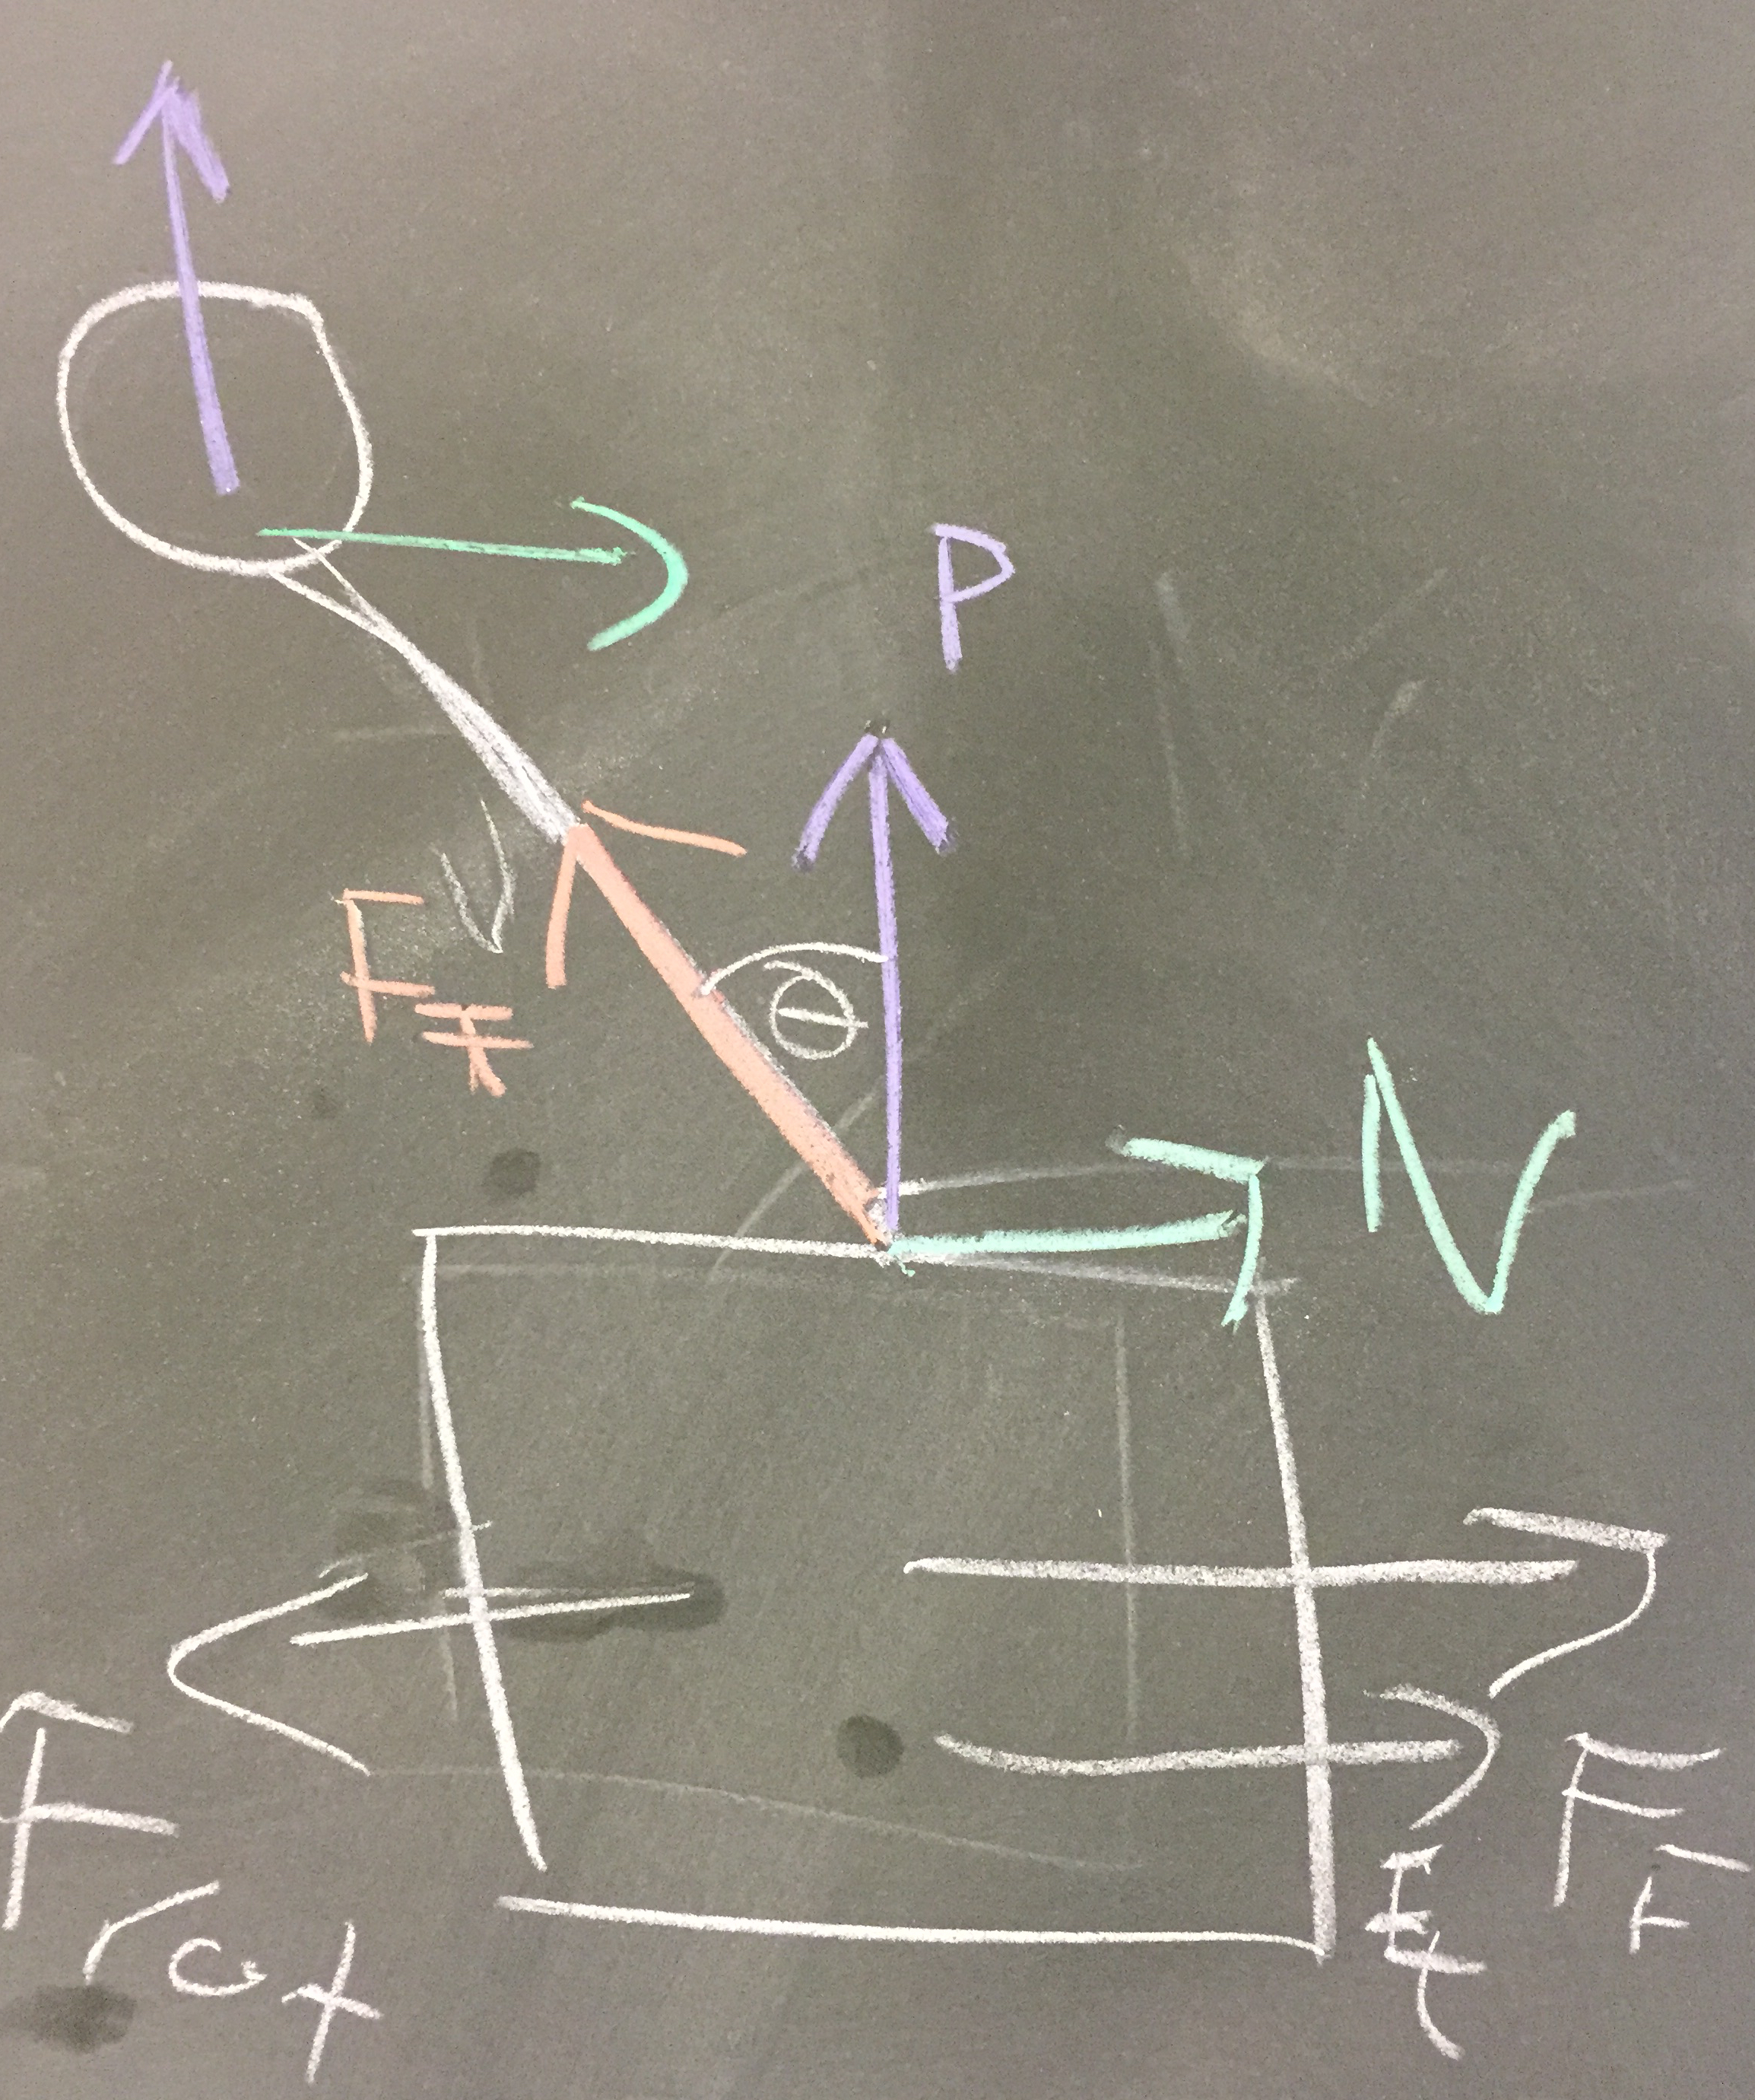
\includegraphics[width =0.3 \textwidth]{figures/inertia11.jpg}
%\caption{Tension force composants.}
%\label{fig:NewFig}
%\end{figure}
%
%From \autoref{fig:NewFig}, it can be seen that the tension force $F_t(\theta_p(t))$ can be slit into two composants, i.e. two forces perpendicular to each other. These can be described as:
%\begin{align}
%F_{t, x}(\theta_p(t)) &= - F_t(\theta_p(t)) \cdot \sin(\theta_p(t))\\
%F_{t, y}(\theta_p(t)) &= F_t(\theta_p(t)) \cdot \cos(\theta_p(t))
%\end{align}
%
%These forces can be used to obtain an expression for the resultant torque acting on the pendulum. From \todo{source: matlab} it can be seen that the following relation applies:
%
%\begin{equation}
%J_p \ddot \theta_p(t) = - F_{t, x}(\theta_p(t)) \cdot l \cdot \cos(\theta_p) - F_{t, y}(\theta_p(t)) \cdot l \cdot \sin(\theta_p)
%\label{inertiaLink}
%\end{equation}
%
%By multiplying \autoref{eom7} with $\cos(\theta_p(t))$ and \autoref{eom8} with $\sin(\theta_p(t))$ then adding the two equations, the expression for the inertia as described in \autoref{inertiaLink} can be utilized, yielding \autoref{eom9}.
%
%Multiply with $l \cdot \cos(\theta)$ on both sides in \autoref{eom7}:
%\begin{align}
%-m_p\cdot l^2 \cdot \ddot \theta_p(t) \cdot \cos^2 (\theta_p(t))+m_p\cdot l^2 \cdot \dot \theta_p^2(t) \cdot \sin(\theta_p(t))\cdot \cos(\theta_p(t))+m_p\cdot l \cdot \ddot x_c \cdot \cos(\theta_p(t)) = F_{t, x}(\theta_p(t)) \cdot l \cdot \sin(\theta_p(t))\label{eom9}
%\end{align}
%
%Multiplying with $l \cdot \sin(\theta)$ on both sides in \autoref{eom8}:
%\begin{align}
%-m_p\cdot l^2 \cdot \ddot \theta_p(t)\cdot \sin^2 (\theta_p(t)) - m_p\cdot l^2 \cdot \dot \theta^2(t) \cdot \cos(\theta_p(t))\cdot \sin(\theta_p(t))=-m_p \cdot l \cdot g\cdot \sin(\theta_p(t)) - F_{t, y}(\theta_p(t)) \cdot l\cdot \sin(\theta_p(t)) \label{eom10}
%\end{align}
%
%Adding \autoref{eom9} and \autoref{eom10} and using the expression for the :
%
%
%
%To eliminate $\ddot x_c(t)$, an equation containing only the variables $\ddot x_c(t)$, $F_F$ and $\theta_p(t)$ and its derivatives must be constructed. This is done by substituting the left side of \autoref{eom7} into \autoref{eom3} in place of $F_t(\theta_p(t)) \cdot sin(\theta_p(t))$. This yields \autoref{eom10}.
%\begin{align}
%(m_p+m_c)\cdot \ddot x_c(t)=m_p\cdot l\cdot \ddot \theta_p(t) \cdot \cos(\theta_p(t))-m_p\cdot l\cdot \dot \theta_p(t)^2 \cdot \sin(\theta_p(t))+F_F(t)\label{eom10}
%\end{align}
%
%With 2 equations containing $\ddot x_c(t)$, this variable is now eliminated by isolating $\ddot x_c(t)$ in \autoref{eom9} and inserting this expression for $\ddot x_c(t)$ in \autoref{eom10}. This yields \autoref{eq:thetaForce}.
%\begin{align}
%\ddot \theta_p(t)(l\cdot (m_p + m_c)-m_p \cdot l \cdot \cos^2(\theta_p(t)))&+\dot\theta_p(t)^2 \cdot (m_p\cdot l\cdot \sin(\theta_p(t))\cdot \cos(\theta_p(t)))\nonumber\\ 
%&=  \\
%\cos(\theta_p(t))\cdot F_F(t)+g\cdot &\sin(\theta_p(t))\cdot (m_p+m_c)\nonumber\label{eq:thetaForce}
%\end{align}
%
%\autoref{eq:thetaForce} contains only two variables, namely $\theta_p(t)$ and $F_F(t)$, thus this single expression describes the motion of the inverted pendulum. This model is clearly not linear, thus it has to be linearised before a transfer function can be determined. This is done in the next subsection.
%
%%In the following section, a block diagram is build from this expression, through which the expression is verified by simulation and subsequent comparison with expected result.
%%changed due to mistak where L was not included.
%%\begin{align}
%%\ddot \theta (-m_1\cdot L \cdot \cos^2(\theta)+(m_1+m_2)\cdot L)+\dot \theta^2(m_1\cdot \sin(\theta)\cdot \cos(\theta))=F_F+(m_1+m_2)\cdot g\cdot \sin(\theta)
%%\end{align}
%The model of the inverted pendulum without the inertia can be expressed as: 
%\begin{equation}
%(m_p+m_c)\cdot \ddot x_c(t)= m_p\cdot l \cdot \ddot \theta_p(t) \cdot \cos(\theta_p(t))-m_p \cdot l \cdot \dot \theta_p(t)^2 \sin(\theta_p(t))+2\cdot F_F(\theta_p(t))\label{eq:penmodelnoinertia}
%\end{equation}
%
%Note, that $F_F(\theta_p(t))$ is multiplied by two, as there are two wheels applying force. \\
%This expression can be combined with \autoref{eq:inertia1}. 
%This is done by isolating $\ddot x_c(t)$ in \autoref{eq:penmodelnoinertia}. Inserting this into \autoref{eq:inertia1} yieds: 
%\begin{align}
%&(J_p+m_p\cdot l^2)\cdot (m_p + m_c)\cdot \ddot \theta_p(t)=(m_p^2 +m_p\cdot m_c)\cdot l \cdot g \cdot \sin(\theta_p(t))\nonumber \\&+m_p^2\cdot l^2\cdot \cos^2(\theta_p(t)) \cdot \ddot \theta_p(t)-m_p\cdot l \cdot \dot \theta_p(t)^2\cdot \sin(\theta_p(t))+2\cdot F_F(\theta_p(t))\label{eq:final_pen22}
%\end{align}
\autoref{eq:model_pen33} and \autoref{eq:inertia1} are the final model expressions for the inverted pendulum. The next step before transfer functions are derived, is to linearize these expressions. This is done in the following section.
\vspace{1 cm}
%This can now be combined with the model expression of the motors and wheels model. This is done in the following section. 
% This will be linearized in the following section and combined with the already linear motormodel. This will lead to a transferfunction for the system, which is to be simulated. From this a controller can be designed and later implemented. 